\section{Background}

	\subsection{Operating Systems}

		% \pholder[Quais modelos existem? Replicado, Mestre-Escravo e Compartilhado]{Multiprocessor Operating Systems}

		\begin{frame}{Types of Operating Systems (OS)}
		\begin{overprint}
			\only<1>{
				\begin{itemize}
					\item Replicated OS
					\item Master-Slave OS
					\item Symmetric OS
				\end{itemize}
				
\includegraphics[width=\linewidth]{imgs/blank-os.pdf}
			}
			\only<2>{
				\begin{itemize}
					\item \textbf{Replicated OS}
					\item Master-Slave OS
					\item Symmetric OS
				\end{itemize}
				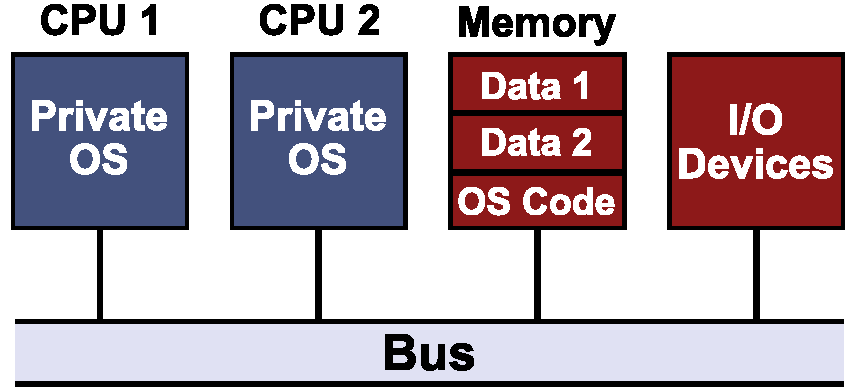
\includegraphics[width=\linewidth]{imgs/replicated-os.pdf}
			}
			\only<3>{
				\begin{itemize}
					\item Replicated OS
					\item \textbf{Master-Slave OS}
					\item Symmetric OS
				\end{itemize}
				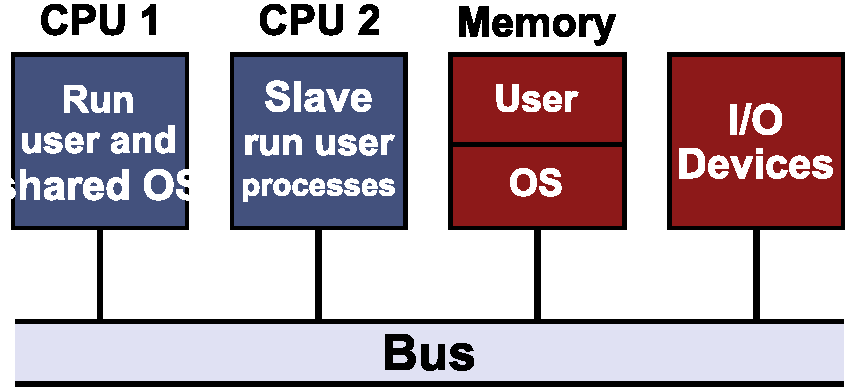
\includegraphics[width=\linewidth]{imgs/master-slave-os.pdf}
			}
			\only<4>{
				\begin{itemize}
					\item Replicated OS
					\item Master-Slave OS
					\item \textbf{Symmetric OS}
				\end{itemize}
				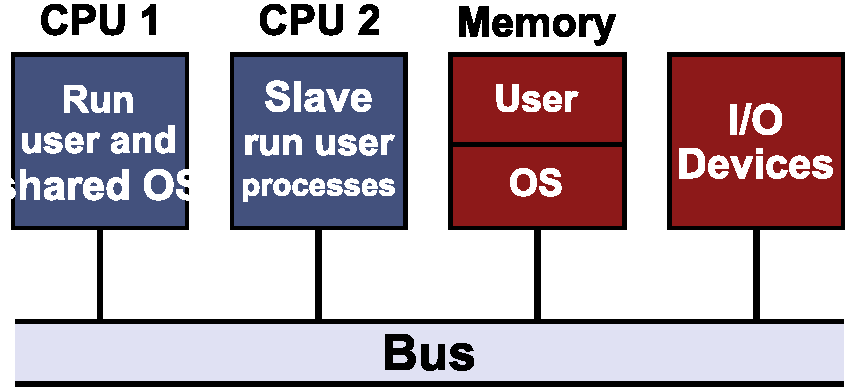
\includegraphics[width=\linewidth]{imgs/master-slave-os.pdf}
			}
		\end{overprint}
		\end{frame}

	\subsection{Message-Passsing Model}

		% \pholder[Software que lida com interfaces e dma?]{Low-Level Communication}
		\begin{frame}[fragile]{Low-Level Communication for Message-Passsing Model}
			\begin{itemize}
				\item Network interfaces
				\item Performance impacts
				\item Direct Memory Access (DMA)
			\end{itemize}
		\end{frame}

		% \pholder[Tipos de envio/recebimento?]{User-Level Communication}
		\begin{frame}[fragile]{User-Level Communication for Message-Passsing Model}
		\begin{overprint}
			\only<1>{
				\begin{itemize}
					\item Send/receive primitives
					\begin{itemize}
						\item Synchronous calls
						\item Asynchronous calls
					\end{itemize}
				\end{itemize}
				
\includegraphics[width=\linewidth]{imgs/call-blank.pdf}
			}
			\only<2>{
				\begin{itemize}
					\item Send/receive primitives
					\begin{itemize}
						\item \textbf{Synchronous calls}
						\item Asynchronous calls
					\end{itemize}
				\end{itemize}
				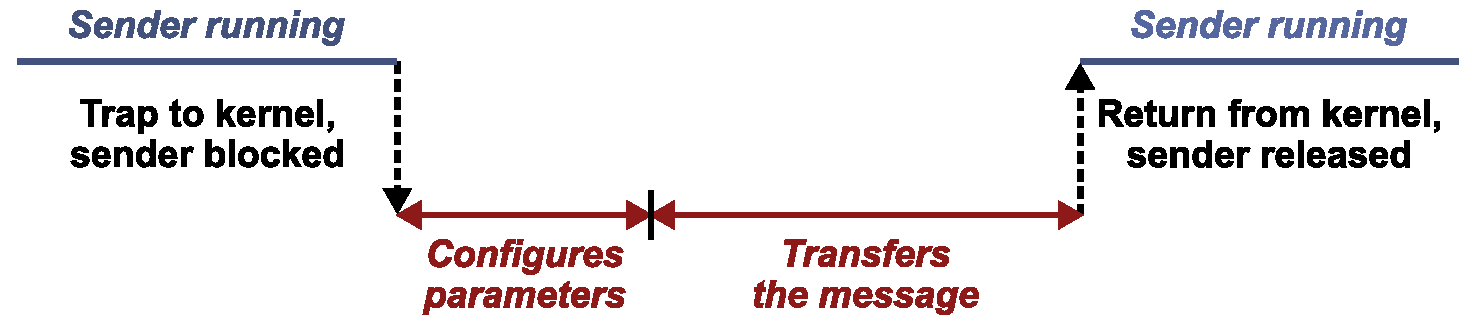
\includegraphics[width=\linewidth]{imgs/call-sync.pdf}
			}
			\only<3>{
				\begin{itemize}
					\item Send/receive primitives
					\begin{itemize}
						\item Synchronous calls
						\item \textbf{Asynchronous calls}
					\end{itemize}
				\end{itemize}
				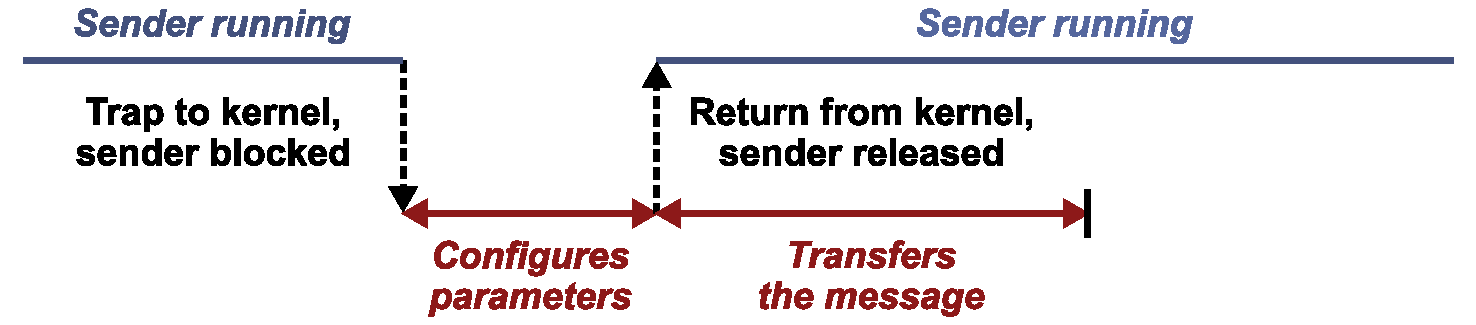
\includegraphics[width=\linewidth]{imgs/call-async.pdf}
			}
		\end{overprint}
		\end{frame}

	\subsection{Kalray MPPA-256}

		% \pholder[Descrever MPPA]{MPPA-256}
		\begin{frame}[fragile]{Kalray MPPA-256}
			\begin{itemize}
				\item {High-Performance and Low-Power Consunption}
				\item {288 processing cores}
				\begin{itemize}
					\item {16 Compute Cluster (CC)}
					\item {4 I/O Cluster (IO)}
				\end{itemize}
				\item {2 NoC's}
				\begin{itemize}
					\item {Data NoC (DNoC)}
					\item {Control NoC (CNoC)}
				\end{itemize}
			\end{itemize}
			\addfig[][width=.5\linewidth]{imgs/arch-mppa.pdf}
		\end{frame}

		\begin{frame}[fragile]{Kalray MPPA-256 Communication Resources}
			\begin{itemize}
				\item 128 slots for receiving commands;
				\item 256 slots for receiving data;
				\item 4 channels for sending commands;
				\item 8 channels for sending data, and;
				\item 8 $\mu$threads for sending asynchronous data.
			\end{itemize}
		\end{frame}

	\subsection{Nanvix OS}

		% \pholder{Nanvix OS}
		\begin{frame}[fragile]{Nanvix OS}
			\addfig[Balance of the Nanvix OS's goals][width=.5\linewidth]{imgs/nanvix-goal.pdf}

			% We believe that significant barriers will still arise in this scenario, and
			% the solution is to rethink \os design from scratch without losing back
			% compatibility~\cite{penna:compas19, penna2019}.

			% The main efforts in \nanvixos are focused on programmability and portability
			% issues of lightweight manycores. This can be accomplished through a fully-featured
			% \posix-compliant \os~\cite{penna:compas19}.

			\begin{itemize}
				\item Nanvix Hardware Abstraction Layer (HAL)
				\item Nanvix Microkernel
				\item Nanvix Multikernel
			\end{itemize}

			% \nanvixos is composed of three distinct kernel layers.
			% In a bottom-up approach of abstraction level, they are namely \textit{\nanvixhal},
			% \textit{\nanvixmicrokernel}, and \textit{\nanvixmultikernel}.
		\end{frame}

		% \pholder{Nanvix HAL}
		\begin{frame}[fragile]{Nanvix HAL}

			\begin{itemize}
				\item Generic and flexible hardware abstraction layer
				\item The layer above the hardware
				\item Standard view of these emerging processors
			\end{itemize}

			\addfig[][width=.6\linewidth]{nanvix-hal-overview.pdf}

			% \nanvixos proposes a generic and flexible \hal around the
			% intrinsic architectural characteristics of the \lightweight \manycores.

			% Unlike other approaches that aim to design a fully-featured \os~\cite{Baumann2009,kluge2014,nightingale2009,rhoden2011},
			% the \nanvixhal belongs to one level below.

			% It is the first layer on top of the hardware and should provide a standard
			% view of these emerging processors for a client application, \eg \os.
			% At this level, we do not protect internal structures with locks.
			% Thus, the upper-level decides how to protect and multiplex \hal access.

			% \autoref{fig:hal-overview} pictures the three logic layers of the \nanvixhal, which are detailed below:

			% \item[Core Abstraction Layer]
			% Encapsula o gerenciamento de um único core, como, rotinas de manutenção da cache
			% e support a tratamento de exceções e interrupções.

			% \item[Cluster Abstraction Layer]
			% Agrupa o gerenciamento de recursos que envolvem todos os núcleos,
			% como memória virutal e notifição entre núcleos.

			% \item[Processor Abstraction Layer]
			% envolve características relacionadas a multiplos clusters,
			% como o módulo de comunicação inter-cluster, foco deste trabalho.
		\end{frame}

		% \pholder{Nanvix Microkernel}
		\begin{frame}[fragile]{Nanvix Microkernel}

			\begin{itemize}
				\item Runs above the Nanvix HAL
				\item Provides bare bones system abstractions
				\item Rich system call interface
				\item Follows a Master-Slave OS model
			\end{itemize}

			\addfig[][width=.6\linewidth]{nanvix-microkernel-overview.pdf}

			% The \textit{\nanvixmicrokernel}, running above the \nanvixhal, provides
			% bare bones system abstractions to the client applications~\cite{penna:sbesc19}.
			% Through a rich system call interface, it follows a Master-Slave \os model
			% to avoid cache coherence issues present in manycores.
			% The scope of the \nanvixmicrokernel is within a single cluster.
			% System calls and internal subsystems manage local and shared resources
			% available to all cores to maintain the coherence of the \os.

			% \item[IPC Facility]
			% 	encapsulates the rest of this undergraduate dissertation, providing
			% 	manipulation and protection of the inter-cluster communication abstractions.

			% \item[Kernel Call Interface]
			% 	isolates the microkernel internal structures through a rich system call interface.
			% 	This interface implements the Master-Slave \os model
			% 	and decides whether or not a kernel call should be executed locally or remotely.
		\end{frame}

		% \pholder{Nanvix Multikernel}
		\begin{frame}[fragile]{Nanvix Multikernel}

			\begin{itemize}
				\item Follows a multikernel design
				\item OS services run in isolation from user processes
				\item User processes request service via message-passing approach
			\end{itemize}

			\addfig[][width=.6\linewidth]{nanvix-multikernel-overview.pdf}

			% The \textit{\nanvixmultikernel} follows a multikernel design, where \os services
			% are scattered across clusters and interact with user processes through a
			% Client-Server model.
			% Ideally, \os services run in isolation from user processes.
			% Via a message-passing approach, user processes request such services and
			% cooperate with other processes.

			% \autoref{fig:multikernel-overview} shows a possible configuration of a
			% manycore using the \nanvixmultikernel.
			% Clusters located at the corners of the processor run kernel services
			% to better serve a nearby subset of clusters.
			% In the other clusters, we can see the distribution of two distinct applications.
			% An application does not necessarily need to use all cores in a cluster.
			% Now, looking carefully at a cluster, we can see that \nanvixmicrokernel
			% always reserves a single core for kernel execution, making the other cores
			% available for application execution.
		\end{frame}

% LocalWords:  template cls standalone GitHub Overleaf bugfixes SVGs
% LocalWords:  Re-empacotamento fontsize Makefile pdflatex imgs PDFs
% LocalWords:  shell-escape frames SVG brazil english lapesd-slides
% LocalWords:  disabletodonotes todonotes TODO's backup showbackup
% LocalWords:  hidebackup abntexcite abntex natbib nobib titleframe
% LocalWords:  frame showsections sidebar stopcountingframes default
% LocalWords:  thanksframe Thank You Questions referencesframe titulo
% LocalWords:  bibfiles pholder todonote placeholder inline addfig
% LocalWords:  opts graphicx addfiglw width Citations dijkstra Direct
% LocalWords:  Closure Parallel dynamic scheduling DoImportantStuff
% LocalWords:  lccp merged cell svg pdf
